

\tikzset{every picture/.style={line width=0.75pt}} %set default line width to 0.75pt        

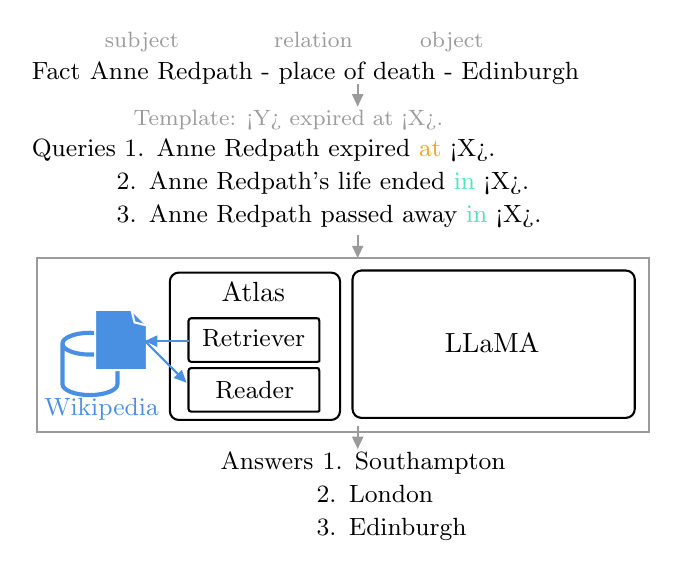
\begin{tikzpicture}[x=0.75pt,y=0.75pt,yscale=-1,xscale=1]
%uncomment if require: \path (0,405); %set diagram left start at 0, and has height of 405

%Rounded Rect [id:dp24858878022074316] 
\draw [shift={(242,173.3)}]  (0,0) .. controls (0,-2.37) and (1.93,-4.3) .. (4.3,-4.3) -- (77.7,-4.3) .. controls (80.07,-4.3) and (82,-2.37) .. (82,0) -- (82,62.4) .. controls (82,64.77) and (80.07,66.7) .. (77.7,66.7) -- (4.3,66.7) .. controls (1.93,66.7) and (0,64.77) .. (0,62.4) -- cycle ;
%Rounded Rect [id:dp150905174339224] 
\draw [shift={(251,192.27)}]  (0,0) .. controls (0,-0.7) and (0.57,-1.27) .. (1.27,-1.27) -- (61.73,-1.27) .. controls (62.43,-1.27) and (63,-1.27) .. (63,0) -- (63,18.46) .. controls (63, 19.16) and (63.43,19.73) .. (61.73,19.73) -- (1.27,19.73) .. controls (0.57,19.73) and (0,19.16) .. (0,18.46) -- cycle ;
%Rounded Rect [id:dp8943318510469378] 
\draw [shift={(251,216.27)}]  (0,0) .. controls (0,-0.7) and (0.57,-1.27) .. (1.27,-1.27) -- (61.73,-1.27) .. controls (62.43,-1.27) and (63,-1.27) .. (63,0) -- (63,18.46) .. controls (63, 19.16) and (63.43,19.73) .. (61.73,19.73) -- (1.27,19.73) .. controls (0.57,19.73) and (0,19.16) .. (0,18.46) -- cycle ;
%Rounded Rect [id:dp43958517904128014] 
\draw [shift={(330,172.3)}]  (0,0) .. controls (0,-2.37) and (1.93,-4.3) .. (4.3,-4.3) -- (131.7,-4.3) .. controls (134.07,-4.3) and (136,-2.37) .. (136,0) -- (136,62.4) .. controls (136,64.77) and (134.07,66.7) .. (131.7,66.7) -- (4.3,66.7) .. controls (1.93,66.7) and (0,64.77) .. (0,62.4) -- cycle ;
%Flowchart: Magnetic Disk [id:dp43919842041587587] 
\draw  [shift={(0,-40)} , color={rgb, 255:red, 74; green, 144; blue, 226 }  ,draw opacity=1 ][fill={rgb, 255:red, 255; green, 255; blue, 255 }  ,fill opacity=1 ][line width=1.5]  (216.75,243.25) -- (216.75,262.75) .. controls (216.75,265.65) and (210.82,268) .. (203.5,268) .. controls (196.18,268) and (190.25,265.65) .. (190.25,262.75) -- (190.25,243.25)(216.75,243.25) .. controls (216.75,246.15) and (210.82,248.5) .. (203.5,248.5) .. controls (196.18,248.5) and (190.25,246.15) .. (190.25,243.25) .. controls (190.25,240.35) and (196.18,238) .. (203.5,238) .. controls (210.82,238) and (216.75,240.35) .. (216.75,243.25) -- cycle ;
%Shape: Folded Corner [id:dp8775935358690414] 
\draw  [shift={(0,-40)} , color={rgb, 255:red, 255; green, 255; blue, 255 }  ,draw opacity=1 ][fill={rgb, 255:red, 74; green, 144; blue, 226 }  ,fill opacity=1 ][line width=0.75]  (223.5,227) -- (206,227) -- (206,256) -- (231,256) -- (231,234.5) -- cycle -- (223.5,227) ; \draw  [shift={(0,-40)} , color={rgb, 255:red, 255; green, 255; blue, 255 }  ,draw opacity=1 ][line width=0.75]  (231,234.5) -- (225,233) -- (223.5,227) ;
%Straight Lines [id:da002595398279400918] 
\draw [shift={(0,-40)} , color={rgb, 255:red, 74; green, 144; blue, 226 }  ,draw opacity=1 ]   (251,242) -- (233,242) ;
\draw [shift={(230,202)}, rotate = 360] [fill={rgb, 255:red, 74; green, 144; blue, 226 }  ,fill opacity=1 ][line width=0.08]  [draw opacity=0] (5.93,-2.79) -- (0,0) -- (5.93,2.79) -- cycle    ;
%Straight Lines [id:da5549948960387789] 
\draw [shift={(0,-40)} , color={rgb, 255:red, 74; green, 144; blue, 226 }  ,draw opacity=1 ]   (230,242) -- (247.88,259.88) ;
\draw [shift={(250,222)}, rotate = 225] [fill={rgb, 255:red, 74; green, 144; blue, 226 }  ,fill opacity=1 ][line width=0.08]  [draw opacity=0] (5.93,-2.79) -- (0,0) -- (5.93,2.79) -- cycle    ;
%Shape: Rectangle [id:dp9473698114792299] 
\draw  [shift={(473,162)}, color={rgb, 255:red, 155; green, 155; blue, 155 }  ,draw opacity=1 ] (-295,0) -- (0,0) -- (0,84) -- (-295,84) -- cycle ;
%Straight Lines [id:da30162599837513593] 
\draw [color={rgb, 255:red, 155; green, 155; blue, 155 }  ,draw opacity=1 ]   (332.5,78) -- (332.5,88) ;
\draw [shift={(332.5,89)}, rotate = 270] [fill={rgb, 255:red, 155; green, 155; blue, 155 }  ,fill opacity=1 ][line width=0.08]  [draw opacity=0] (5.93,-2.79) -- (0,0) -- (5.93,2.79) -- cycle    ;
%Straight Lines [id:da9111484431566645] 
\draw [color={rgb, 255:red, 155; green, 155; blue, 155 }  ,draw opacity=1 ]   (332.5,151) -- (332.5,159) ;
\draw [shift={(332.5,162)}, rotate = 270] [fill={rgb, 255:red, 155; green, 155; blue, 155 }  ,fill opacity=1 ][line width=0.08]  [draw opacity=0] (5.93,-2.79) -- (0,0) -- (5.93,2.79) -- cycle    ;
%Straight Lines [id:da5601546461770723] 
\draw [shift={(0,-40)}, color={rgb, 255:red, 155; green, 155; blue, 155 }  ,draw opacity=1 ]   (332.5,283) -- (332.5,291) ;
\draw [shift={(332.5,254)}, rotate = 270] [fill={rgb, 255:red, 155; green, 155; blue, 155 }  ,fill opacity=1 ][line width=0.08]  [draw opacity=0] (5.93,-2.79) -- (0,0) -- (5.93,2.79) -- cycle    ;
% Text Node
\draw (174,66) node [anchor=north west][inner sep=0.75pt]   [align=left] {{\small Fact} {\small Anne Redpath - place of death - Edinburgh}};
% Text Node
\draw (174,103) node [anchor=north west][inner sep=0.75pt]   [align=left] {{\small Queries 1.} {\small Anne Redpath expired \textcolor[rgb]{0.96,0.65,0.14}{at} <X>.} \\{\small \hspace{0.97cm} 2.} {\small Anne Redpath's life ended \textcolor[rgb]{0.31,0.89,0.76}{in} <X>.}\\{\small \hspace{0.97cm} 3.} {\small Anne Redpath passed away \textcolor[rgb]{0.31,0.89,0.76}{in} <X>.}{\small  }};
% Text Node
\draw (265,254) node [anchor=north west][inner sep=0.75pt]   [align=left] {{\small Answers} 	{\small 1.} {\small Southampton} \\ {\small \hspace{1.11cm} 2.} {\small London} \\{\small \hspace{1.11cm} 3.} {\small Edinburgh} {\small  }};
% Text Node
\draw (208,51.5) node [anchor=north west][inner sep=0.75pt]  [color={rgb, 255:red, 155; green, 155; blue, 155 }  ,opacity=1 ] [align=left] {\begin{minipage}[lt]{28.58pt}\setlength\topsep{0pt}
\begin{center}
{\footnotesize subject}
\end{center}

\end{minipage}};
% Text Node
\draw (290,51.5) node [anchor=north west][inner sep=0.75pt]  [color={rgb, 255:red, 155; green, 155; blue, 155 }  ,opacity=1 ] [align=left] {\begin{minipage}[lt]{29.48pt}\setlength\topsep{0pt}
\begin{center}
{\footnotesize relation}
\end{center}

\end{minipage}};
% Text Node
\draw (360,51.5) node [anchor=north west][inner sep=0.75pt]  [color={rgb, 255:red, 155; green, 155; blue, 155 }  ,opacity=1 ] [align=left] {\begin{minipage}[lt]{24.5pt}\setlength\topsep{0pt}
\begin{center}
{\footnotesize object}
\end{center}

\end{minipage}};
% Text Node
\draw (265.5,172) node [anchor=north west][inner sep=0.75pt]  [color={rgb, 255:red, 0; green, 0; blue, 0 }  ,opacity=1 ] [align=left] {Atlas};
% Text Node
\draw (254.21,195) node [anchor=north west][inner sep=0.75pt]   [align=left] {\begin{minipage}[lt]{39.96pt}\setlength\topsep{0pt}
\begin{center}
{\small Retriever}
\end{center}

\end{minipage}};
% Text Node
\draw (259.5,220) node [anchor=north west][inner sep=0.75pt]   [align=left] {\begin{minipage}[lt]{32.83pt}\setlength\topsep{0pt}
\begin{center}
{\small Reader}
\end{center}

\end{minipage}};
% Text Node
\draw (373,197) node [anchor=north west][inner sep=0.75pt]  [color={rgb, 255:red, 0; green, 0; blue, 0 }  ,opacity=1 ] [align=left] {LLaMA};
% Text Node
\draw (180,228) node [anchor=north west][inner sep=0.75pt]  [font=\small,color={rgb, 255:red, 74; green, 144; blue, 226 }  ,opacity=1 ] [align=left] {Wikipedia};
% Text Node
\draw (223,89) node [anchor=north west][inner sep=0.75pt]  [font=\footnotesize,color={rgb, 255:red, 155; green, 155; blue, 155 }  ,opacity=1 ] [align=left] {Template:  <Y> expired at <X>.};


\end{tikzpicture}
